\chapter{JavaScript eta DOM}

DOM, \textit{Document Object Model} edo Dokumentuaren Objektu Eredua XML edo HTML dokumentu bat hainbat nodoz osatutako zuhaitz-egitura bat bezala tratatzen duen interfazea da.  Nodo bakoitzean dokumentuaren zati bat irudikatzen duen objektu bat dago. Beste era batera esanda, DOM interfazeak dokumentu bat zuhaitz logiko batez irudikatzen du.  DOM eredua JavaScript bidez nola atzitu eta nola alda dezakegun ikasiko dugu gai honetan, modu dinamikoan web orri baten edukia aldatu ahal izateko. 

Zuhaitz logiko horren barruan dauden objektuak JavaScript erabiliz atzitu, irakurri, aldatu edo ezabatu ditzakegu.
Nabigatzaileak automatikoki eta berehala interpretatuko ditu DOM zuhaitzean egindako aldaketak.

Adibide batekin ikusiko dugu. Demagun HTML orri soil hau kargatu nahi dugula:

\begin{lstlisting}[language=HTML,numbers=none]
<!DOCTYPE html>
<html>
<head>
<title>My title</title>
</head>
<body>
<h1>A heading</h1>
<a HREF="">Link text</a>
</body>
</html>
\end{lstlisting}


Horri dagokion DOM zuhaitza \ref{fig:DOM}. irudian ikus dezakegu.

\begin{figure}[ht]
	\centering
\begin{tikzpicture}
\node[anchor=south west,inner sep=0] (image) at (0,0)
   {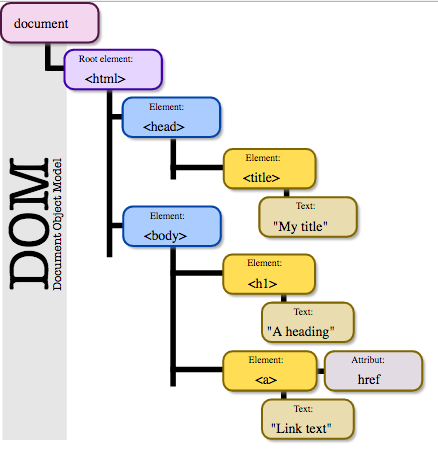
\includegraphics[trim=0cm 0cm 0cm 0cm, clip=true, width=0.5\textwidth]{img/DOM}};
\end{tikzpicture}
\caption{DOM Eredua. Iturria: \newline
\href{http://upload.wikimedia.org/wikipedia/commons/5/5a/DOM-model.svg}{http://upload.wikimedia.org/wikipedia/commons/5/5a/DOM-model.svg}.}
\label{fig:DOM}
\end{figure}

\section{DOM aldatzen JS bidez}

Demagun \ref{fig:ariketaDOM}. irudiko DOM zuhaitza dugula. Bertan, JS erabiliz, hirugarren paragrafoaren (\hl{<p>}) testua aldatu nahi dugu, \textquotedbl{}estás\textquotedbl{} jarri ordez, \textquotedbl{}zaude?\textquotedbl{} ager dadin. Nola egin?

\index{getElementById()}
Lehenengo \textit{hiru} izeneko identifikatzailea duen objektua atzituko dugu,
\index{innerHTML} \hl{document.getElementById()} metodoaz. Metodo horrek DOM zuhaitza zeharkatuko du parametro gisa pasatu diogun identifikatzailea bilatuz. Identifikatzailea bakuna denez, soilik elementu bat aurkituko du. Objektu horrek hainbat metodo eta atributu izango ditu, adibidez \textquotedbl{}innerHTML\textquotedbl{} atributua, objektuaren barruko HTMLa atzitu edo editatzeko aukera emango diguna. Beraz, \textquotedbl{}estás\textquotedbl{} hitza \ref{list:ariketaDOM}. listatuko kodearekin lortu beharko genuke. Probatuko dugu ea egia den...

\begin{figure}[ht]
	\centering
\begin{tikzpicture}
\node[anchor=south west,inner sep=0] (image) at (0,0)
   {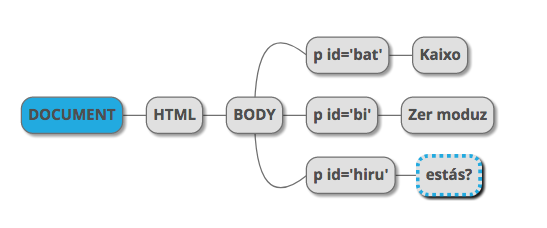
\includegraphics[trim=0cm 0cm 0cm 0cm, clip=true, width=0.5\textwidth]{img/DOMAriketa}};
\end{tikzpicture}
\caption{DOM interfazea ulertzeko ariketaren testuingurua.}
\label{fig:ariketaDOM}
\end{figure}


\begin{lstlisting}[language=JavaScript,numbers=none, label={list:ariketaDOM}, caption={getElementById erabil dezakegu DOM zuhaitzeko objektu bat atzitzeko.}]
let osagai = document.getElementById("hiru");
osagai.innerHTML = "zaude?";
\end{lstlisting}

\section{Nola txertatu JS script bat zure orrian}
Aurreko kodea index.html izeneko orri batean txerta dezakegu. Bi modu daude, \textit{inline} deritzona edo erreferentzia gisa. \index{inline}

\begin{lstlisting}[language=JavaScript,label={list:inlinejs}, caption={\textit{inline} izeneko moduan kodea zuzenean txertatzen da <script> etiketen artean. Ikus: \href{https://codesandbox.io/s/4-gaia-dom-k701t?file=/index.html}{https://codesandbox.io/s/4-gaia-dom-k701t?file=/index.html}}.]
<!DOCTYPE html>
<html lang="eu-es">
  <head>
    <meta charset="utf-8" />
    <script>
      let osagai = document.getElementById("hiru");
      osagai.innerHTML = "zaude?";
    </script>
  </head>
  <body>
    <p id="bat">Kaixoooo</p>
    <p id="bi">Zer moduz</p>
    <p id="hiru">estás?</p>
  </body>
</html>
\end{lstlisting}

\begin{lstlisting}[language=HTML,label={list:referencejs}, caption={JS kodea erreferentziaz ere txerta dezakegu. Horretarako, JS fitxategiaren izena pasatuko diogu <script> etiketari, src atributuan}.]
<!DOCTYPE html>
<html lang="eu-es">
  <head>
    <meta charset="utf-8" />
    <script src="scripta.js"></script>
  </head>
  <body>
    <p id="bat">Kaixoooo</p>
    <p id="bi">Zer moduz</p>
    <p id="hiru">estás?</p>
  </body>
</html>
\end{lstlisting}

Bi kode zati horiek probatuz gero, funtzionatzen ez dutela ikusiko dugu (ikus \ref{fig:no-onload}. irudia). Zergatik? Nabigatzaileak ikusi eta exekutatu duen lehenengo gauza (kodea irakurriz goitik hasita) <head> blokean dagoena delako. Bertan gure <script>-a exekutatu du, baina oraindik ez du orriaren gorputza (body-a) kargatu! Hori dela eta, ezin du aldaketarik egin. Izan ere, kontsola irekitzen badugu, honako errorea ikusiko dugu:

\begin{lstlisting}[language=JavaScript,numbers=none]
Uncaught TypeError: Cannot set property 'innerHTML' of null at (index):9
\end{lstlisting}
    
Alegia, nabigatzailea saiatu da osagaia aurkitzen \textit{document.getElementById("hiru")} eginez, baina ez du ezer topatu. Beraz, \textit{osagai = null} da, eta, hortaz, 
\textit{osagai.innerHTML = "zaude?";} egiten saiatzean, errorea.

\index{onload}
Nola konpondu? Nola esan diezaiokegu nabigatzaileari JavaScript kodea orriaren gorputza kargatu eta gero exekutatu behar duela? Horretarako jaio zen \hl{onload} gertaera-kudeatzailea. Azter dezagun hurrengo atalean.

\begin{figure}[ht]
	\centering
\begin{tikzpicture}
\node[anchor=south west,inner sep=0] (image) at (0,0)
   {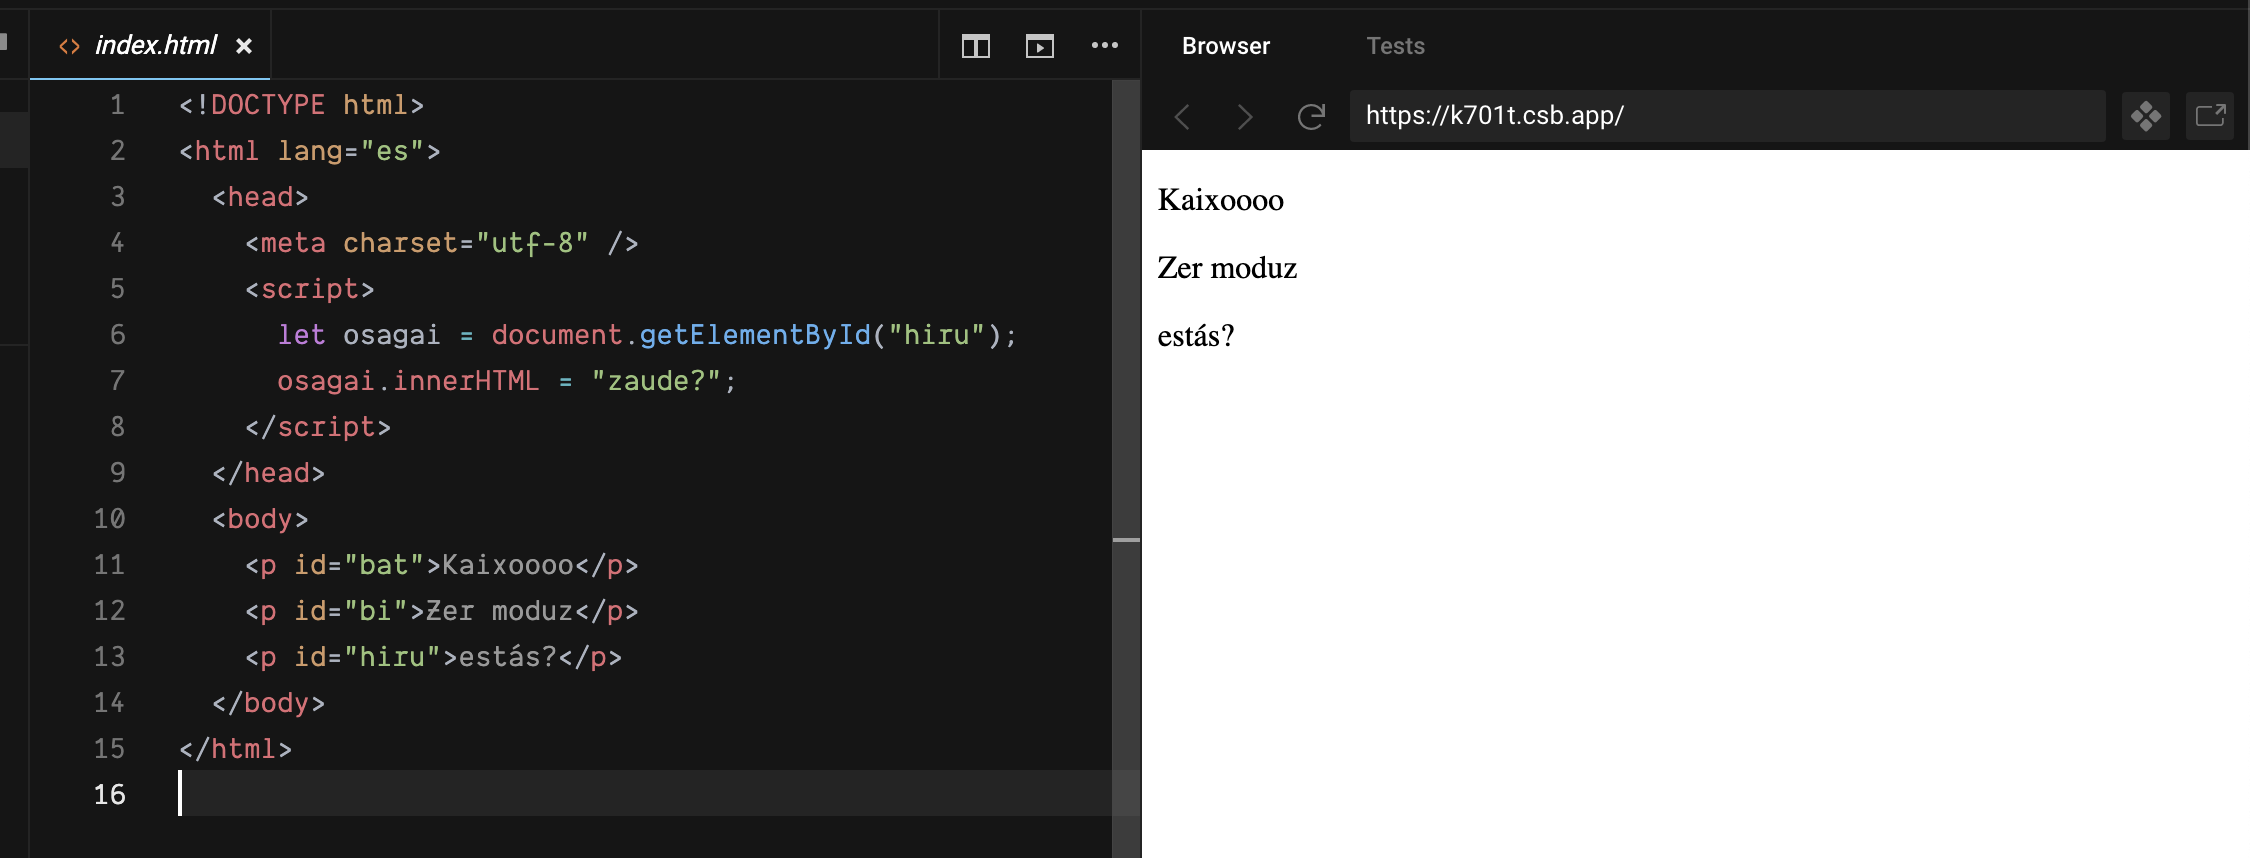
\includegraphics[trim=0cm 0cm 0cm 0cm, clip=true, width=1.0\textwidth]{img/4gaia-no-onload.png}};
\end{tikzpicture}
\caption{DOM edukia aldatzen saiatu gara, baina ez dugu lortu. Zergatik izango ote da... Gai honetan  azalduko dugu.}
\label{fig:no-onload}
\end{figure}

\subsection{onload gertaera-kudeatzailea}

\begin{lstlisting}[language=HTML,label={list:onloadjs}, caption={window.onload egitean gertaera-kudeatzaile bat ezartzen ari gara. Kasu honetan kudeatzailea orriaren edukia kargatu ostean exekutatu egin behar dela esaten ari gara. Ikus: \href{https://codesandbox.io/s/4-gaia-onload-x7wkr?file=/index.html}{https://codesandbox.io/s/4-gaia-onload-x7wkr?file=/index.html}}.]
<!DOCTYPE html>
<html lang="eu-es">
  <head>
    <meta charset="utf-8" />
    <script>
      function edukiaAldatu() {
        let osagai = document.getElementById("hiru");
        osagai.innerHTML = "zaude?";
      }
      window.onload = edukiaAldatu;
    </script>
  </head>
  <body>
    <p id="bat">Kaixoooo</p>
    <p id="bi">Zer moduz</p>
    <p id="hiru">estás?</p>
  </body>
</html>
\end{lstlisting}


\textit{Window} objektuak onload gertaera-kudeatzailea dauka, besteak beste (\textit{window.onload}). Horri esker nabigatzailearen portaera kudea dezakegu. Zehazki, orriaren edukia kargatzen bukatzen denean, \textit{loaded} gertaera altxatuko da. Gertaera hori antzeman eta \hl{edukiaAldatu} izeneko funtzioarekin tratatu nahi dugula esaten ari gara lerro honekin:

\begin{lstlisting}[language=JavaScript, numbers=none]
   window.onload = edukiaAldatu;
\end{lstlisting}

Noski, DOM edukia aldatzeko prestatuta genuen kodea orain \hl{edukiaAldatu} izeneko funtzioan sartu dugu:

\begin{lstlisting}[language=JavaScript]
 function edukiaAldatu() {
        let osagai = document.getElementById("hiru");
        osagai.innerHTML = "zaude?";
      }
\end{lstlisting}

Eta orain bai, dena ondo dabil (ikus \ref{fig:onload}. irudia). Gertaera mota ezberdin interesgarri askoz gehiago daude. Izan ere, horretarako beste gai bat bereziki prestatu dugu liburu honetan (ikus \textbf{6. Gertaerak} kapitulua).

\begin{figure}[ht]
	\centering
\begin{tikzpicture}
\node[anchor=south west,inner sep=0] (image) at (0,0)
   {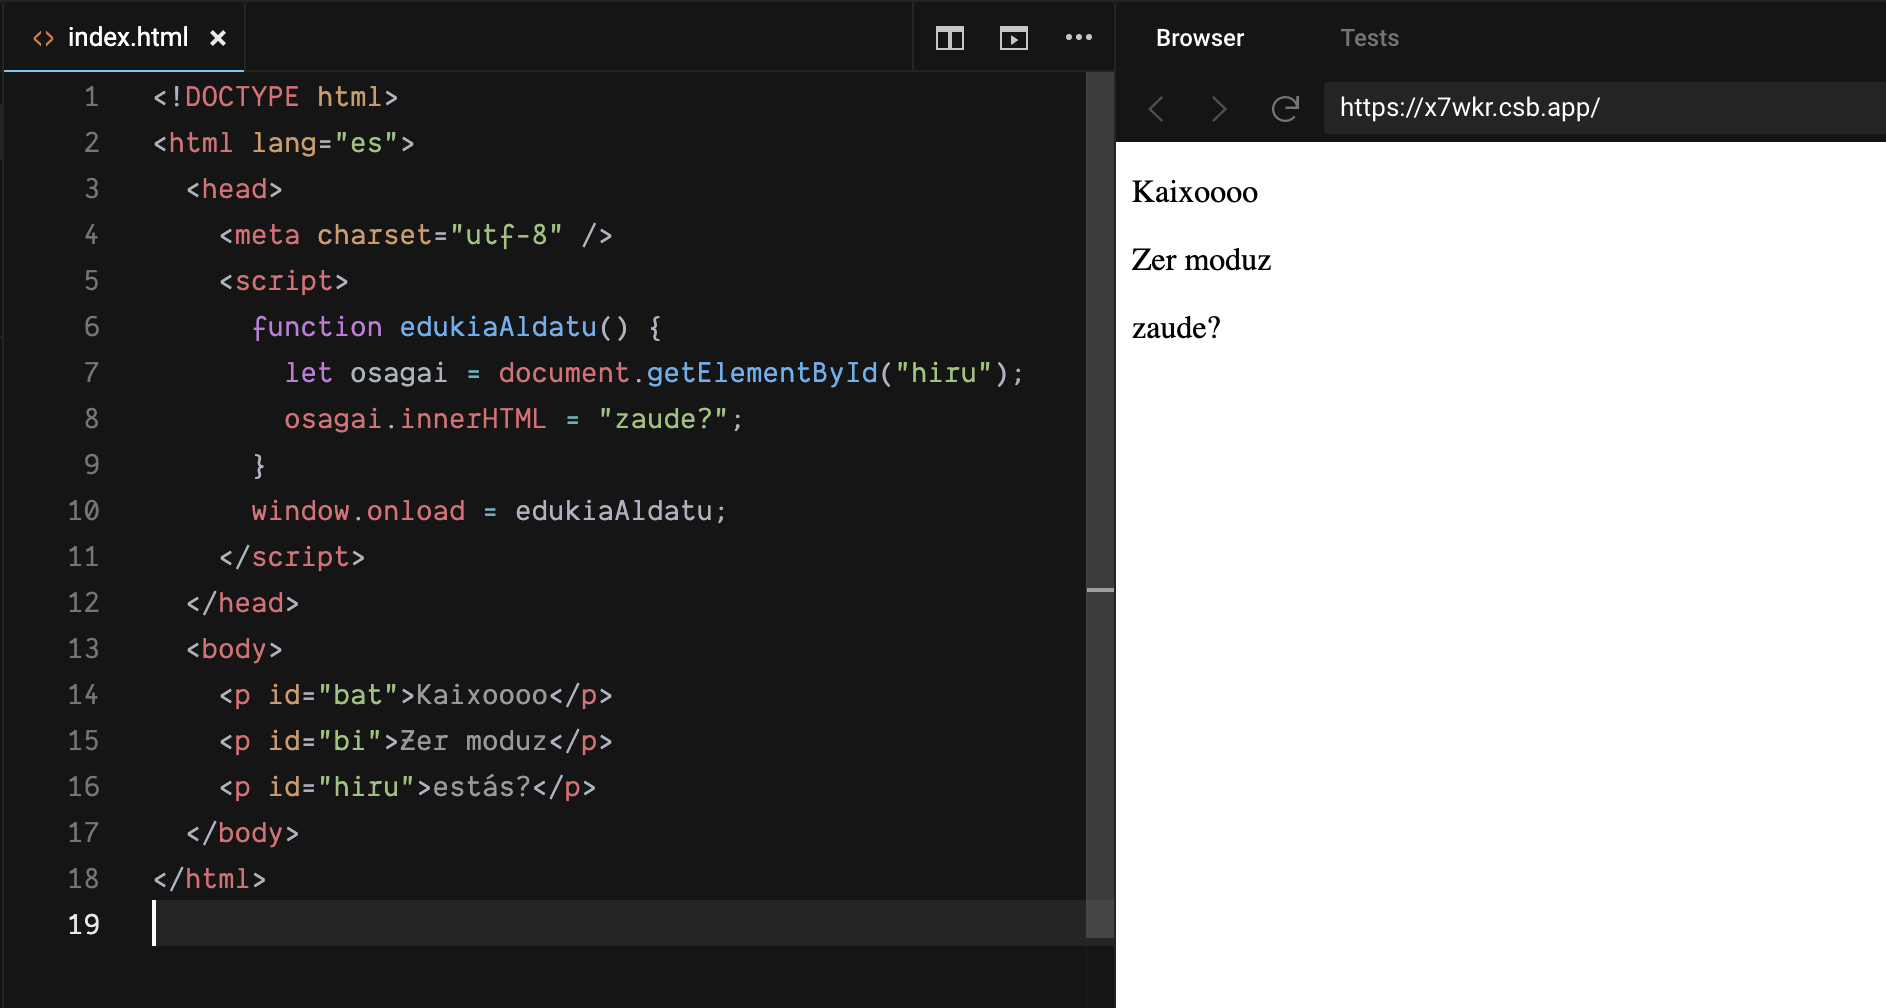
\includegraphics[trim=0cm 0cm 0cm 0cm, clip=true, width=1.0\textwidth]{img/4gaia-onload.png}};
\end{tikzpicture}
\caption{DOM edukia aldatzeko, lehenengo eta behin, orriaren edukia kargatu behar da. Hori lortzeko \textit{window.onload} gertaera-kudeatzailea prestatu dugu.}
\label{fig:onload}
\end{figure}


\section{Ariketak}

Esteka honetan \href{https://labur.eus/WOXzZ}{https://www.dropbox.com/s/7kq7nm8j6m3o9zh/initializr.tgz?dl=1} hurrengo ariketa egiteko beharrezkoak diren fitxategiak aurkituko
dituzu. Jaitsi, destrinkotu eta zure nabigatzailean
index.html orria ireki.

Bertan, webgune baten HTML kodea ematen zaizu. Zure eginbeharra: JS \mbox{script} baten bidez orri nagusian dagoen goiburua ordezkatu, "Uno", "Dos", \mbox{\textquotedbl{}Three\textquotedbl{}} katearen ordez \textquotedbl{}Bat\textquotedbl{}, \textquotedbl{}Bi\textquotedbl{}, \textquotedbl{}Hiru\textquotedbl{} katea ager dadin.

\begin{figure}[ht]
	\centering
\begin{tikzpicture}
\node[anchor=south west,inner sep=0] (image) at (0,0)
   {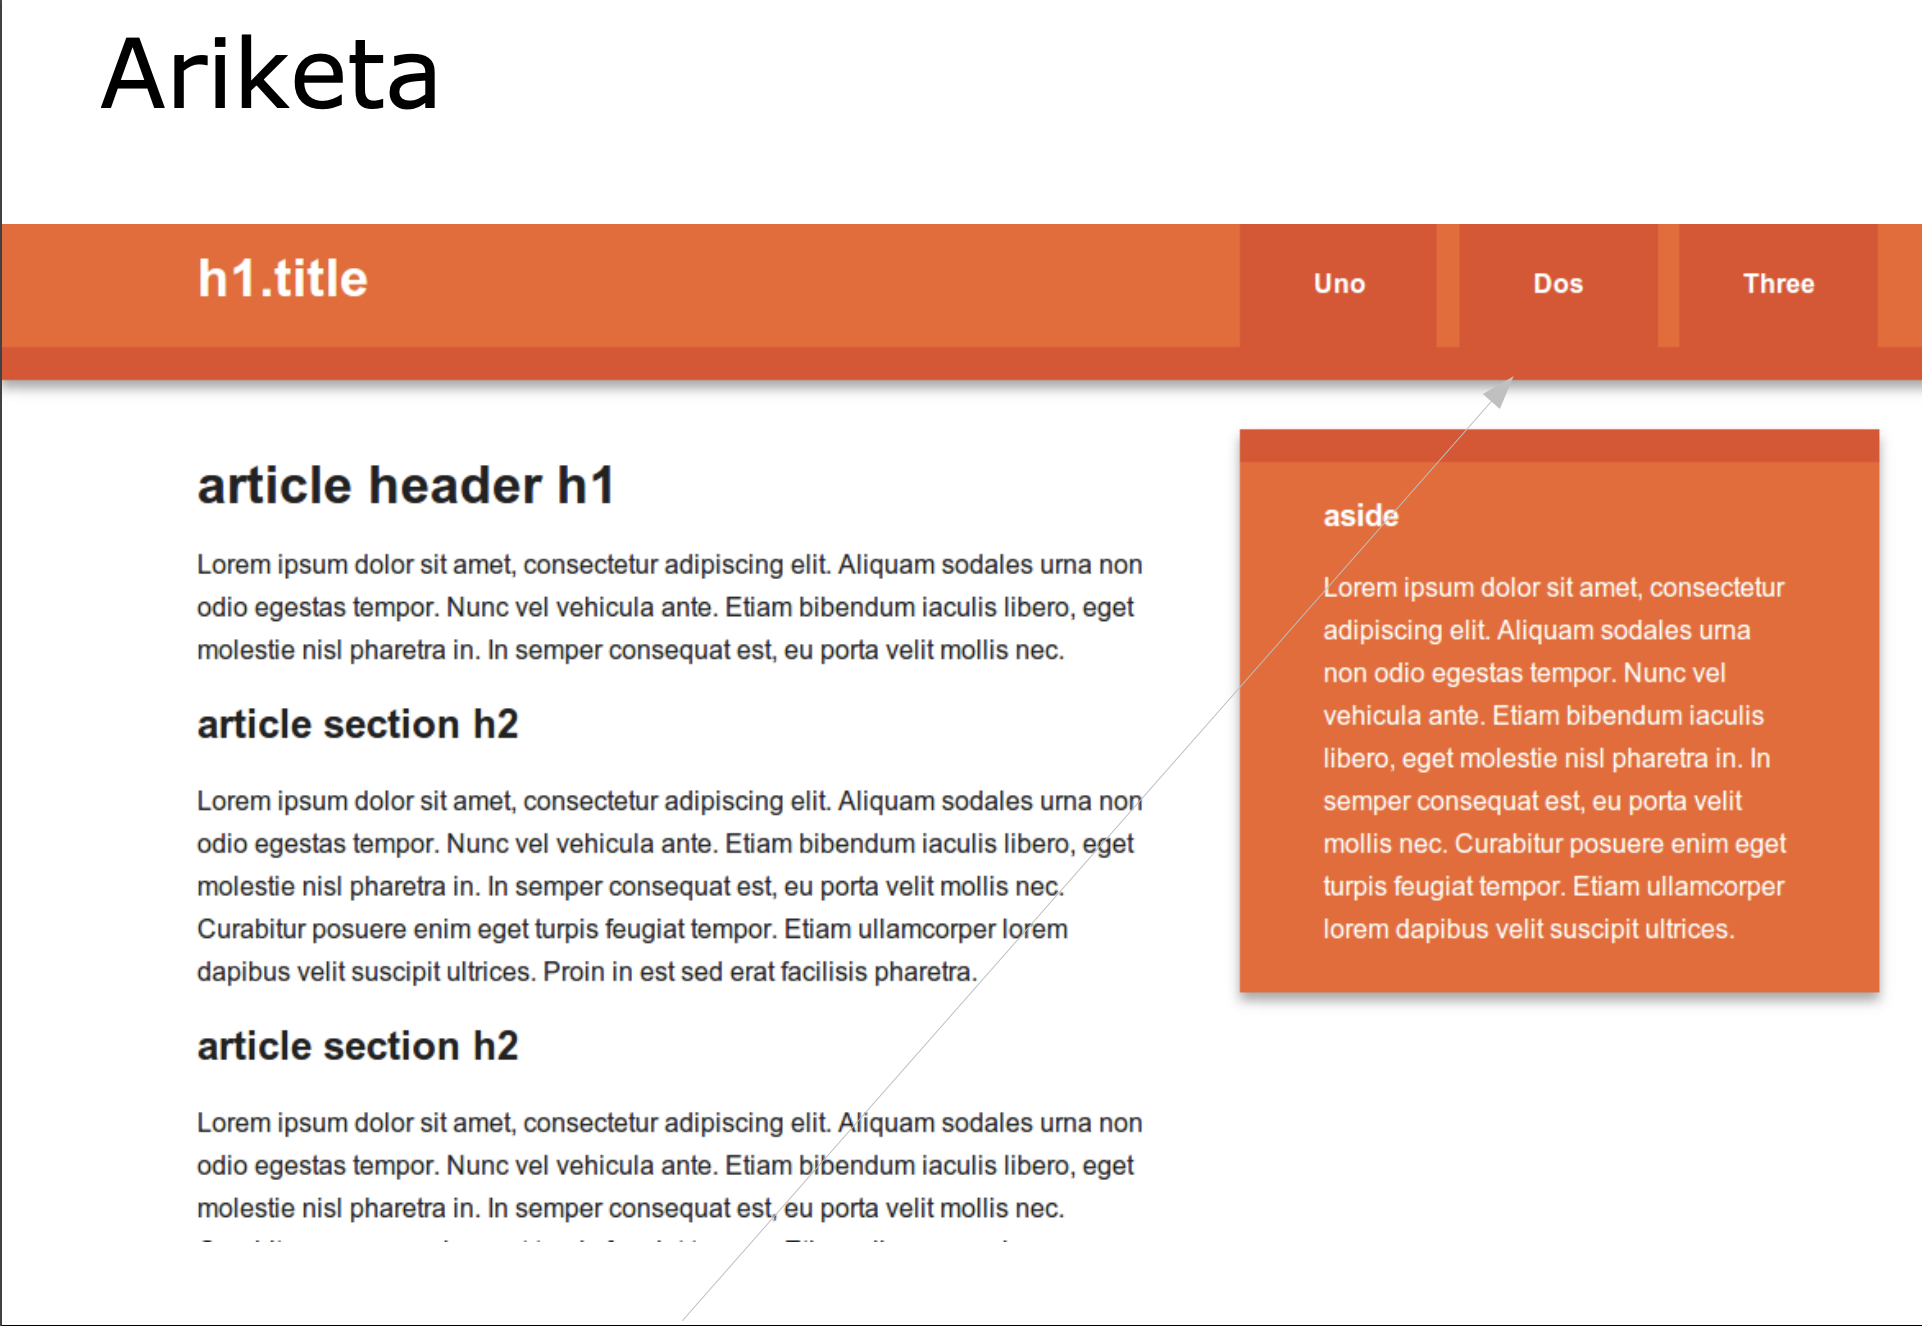
\includegraphics[trim=0cm 0cm 0cm 0cm, clip=true, width=.75\textwidth]{img/dom_ariketa.png}};
\end{tikzpicture}
\caption{DOM edukia aldatzeko JS bat prestatu beharko duzu.}
\label{fig:onload}
\end{figure}